\newpage
\section{Sømløs kloning}
\label{sec:kloning}
\subsection{Bakgrunn}
En populær anvendelse av Poisson-problemet er sømløs kloning. Det går ut på å flytte en partisjon av et bilde over i et annet med den hensikt å minimalisere synligheten av overgangen mellom dem. De fleste profesjonelle bilderedigeringsverktøy har en form for sømløs kloning implementert. Her gjøres operasjonene grafisk ved hjelp av noen museklikk, men i bakgrunnen ligger altså en kode ikke altfor ulik den som er implementert her.\newline
Problemet kan formuleres som et Poisson-problem dersom $u_0$ er originalbildet det skal klones inn i, og $u_1$ bildet utsnittet skal hentes fra. Problemstillingen blir da å finne $u$ slik at $u=u_0$ utenfor masken $\Omega_i$ og $\nabla^2 u = \nabla^2 u_1$ i $\Omega_i$. Dette kan løses ved Poisson-likningen (\ref{eq:diffusjon}) ved å sette $h=\nabla^2 u_1$, med Dirichlet randbetingelser: $u=u_0$ på $\partial \Omega_i$. 

\subsection{Implementasjon}
Først må en velge to bilder hvor deler av det ene skal flyttes inn i det andre. Deretter må en lage en partisjon av bildet man vil lime inn deler av. Dette har vi implementert ved å definere utsnittet som et rektangel. Deretter hentes \texttt{laplace1} fra $u_1$ før (\ref{eq:diffusjon}) løses med \texttt{h=laplace1}:

\begin{lstlisting}[language=Python]
for i in range(1000):
    laplace2 = (im_ed[0:-2, 1:-1] +              # Laplace for likning 2
                im_ed[2:, 1:-1] +    
                im_ed[1:-1, 0:-2] +
                im_ed[1:-1, 2:] -
                4 * im_ed[1:-1, 1:-1])
    im_ed[1:-1, 1:-1]+=alpha*(laplace2-laplace1) # Los diffusjonslikningen
\end{lstlisting}
Resultatet ved å velge et område på $u_0$ som samsvarer noenlunde med fargene og objektene fra $u_1$ vises i Figur \ref{fig:seamless}. Her fører de sømløse overgangene mellom de to bildene til at det er vanskelig å se hvor skillet går med det blotte øyet. 
\begin{figure}[H]
\begin{center}
    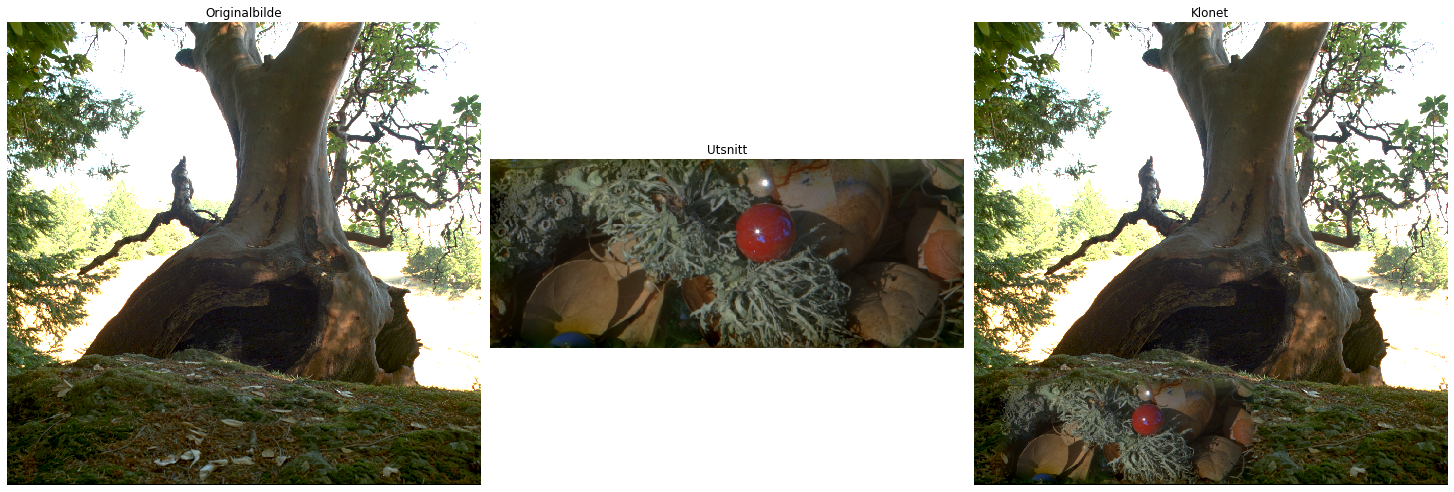
\includegraphics[width=1\columnwidth]{bilder/kloning.png}
    \caption{Sømløs kloning
    \label{fig:seamless}} 
\end{center}
\end{figure}

